%\subsection{Use case}
\subsection{Case study}

\emph{Description}: \cmt{The use case scenario (\fig{fig:usecase:cranes}) \cite{cps4eu2022} involves the process of lifting a platform using drones without human intervention. The cranes use sophisticated automation to perform lifting tasks with minimal human intervention. The project utilizes drones to synchronize the lifting operation between cranes. At each time unit \emath{H}, the drone sends a lifting measurement to one crane in order to stabilize the platform. The platform is equipped with two markers scanned by the drone to calculate their distance from the ground. The resulting lifting distance is then sent as a payload message to one crane until an optimal position for the platform is reached. The operation necessitates the involvement of an edge gateway responsible for clock synchronization. Additionally, one of the drones is particularly sensitive to environmental conditions, which can result in the discussed clock drift, as mentioned in the previous sections.} 


As outlined in \cite{Cockburn2000}, the process flow is described as follows:
\noindent
\begin{figure}[!htbp]
    \centering
    		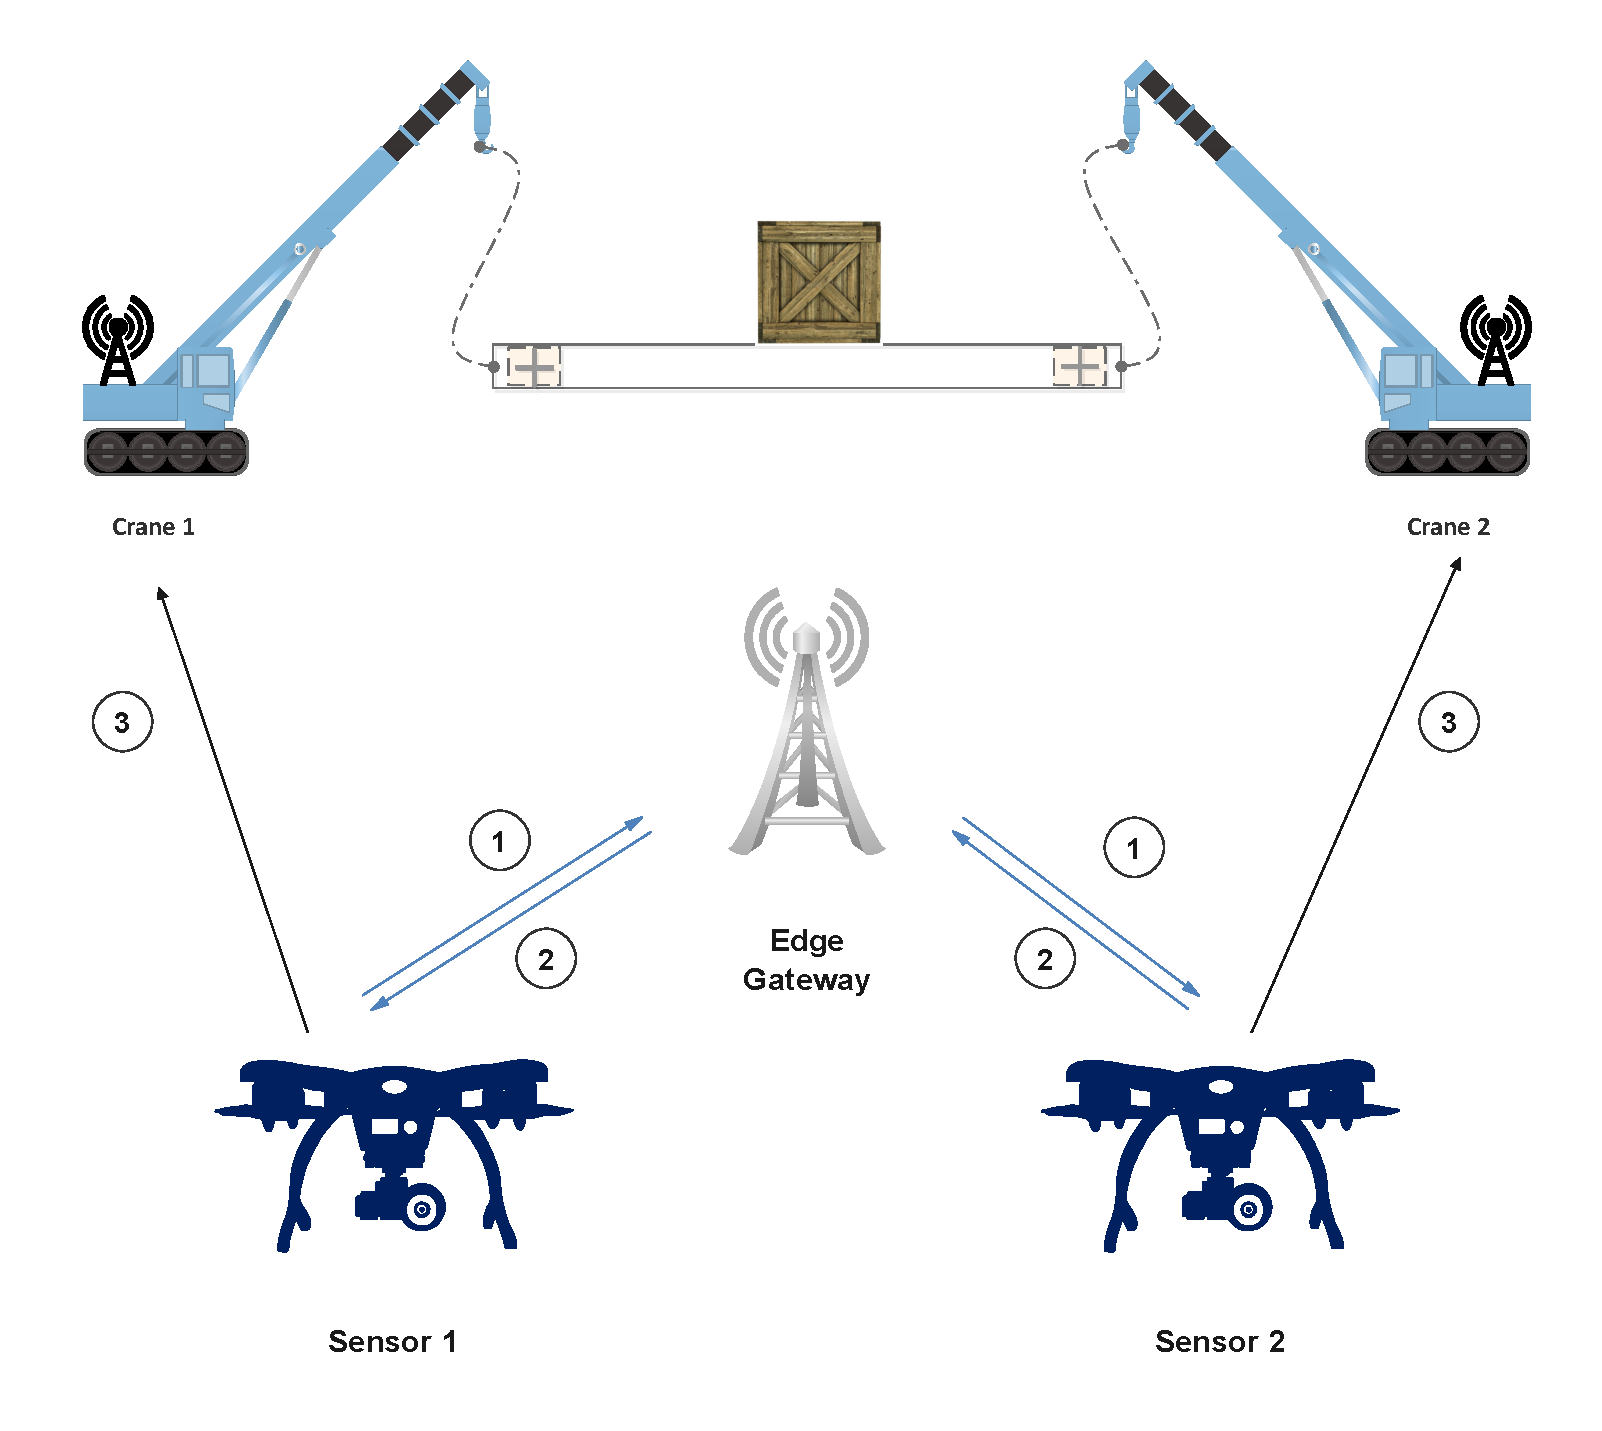
\includegraphics[width=250pt, height =200pt]{uc.pdf}
    \caption{Cranes Lifting Orchestration via a Drone \cite{cps4eu2022}. }
    \label{fig:usecase:cranes}
\end{figure} 


\emph{Actor}: Drone Operator, Crane Operator.

\emph{Preconditions}:
\begin{itemize}
    \item A stable landing pad for drones has been set up.
    \item One drone is available for operation.
    \item Cranes have been positioned at strategic locations around the site.
\end{itemize}
    
\emph{Basic Flow}:
\begin{itemize}
    \item  \circled{1} The drone operator initializes communication messaging between drones and the gateway.
    \item At each time unit \emath{H}, the drone sends its internal clock ticks value to the edge and then receives the average values \circled{2}.    
    \item The drone scans two markers on the lift system's platform and calculates their distance from the ground level.
    \item Using this information, \circled{3} they send a payload message containing calculated lift measurements required by different cranes involved in stabilizing operations. 
    \item Crane operators receive these messages and adjust their equipment accordingly. 
     \item The process repeats iteratively until optimal positioning has been achieved through the refinement of lift measurements communicated between these two systems.
\end{itemize}
\emph{Post-Conditions}: 
\begin{itemize}
\item The lift operation was completed successfully without any damages or accidents. 
\item The cargo was safely lifted onto its designated location.
\end{itemize}

\paragraph{Experimental setup}
We used PRISM v4.7 for our analysis.  The experiments were conducted on an Ubuntu-I7 system with 32GB of RAM. The system models are available online \cite{csi2023}, with references  \eclipse{M1} to \eclipse{M6}. The engine is set to \quot{Explicit}; PRISM supports other computation engines (MTBDD, sparse, and hybrid) that offer different performances regarding model and properties structure (Please refer to documentation in \cite{prism-engines}). Rewards properties are not supported by the \quot{Explicit} engine. A Python code was developed to learn PDT based on the generated OMNeT++ dataset and mapped it to the PRISM code under reference \eclipse{P2}. We describe the desired properties of our models in the Modeling section.

\paragraph{Artefacts}
The experiments detailed in this section are both publicly available and fully reproducible. The source code in PRISM and OMNeT++ can be accessed from the public GitHub repository \cite{csi2023}. The website includes instructions for setting up and running the experiments and how to use the OMNeT++ execution trace data.



\subsection{Drones and InBox behavior modeling}
The modeled system for drone behavior is depicted in Algorithm \ref{algo:model:algo:figo}. The algorithm is structured with if-then-else statements that must be translated into PRISM commands. This translation is based on personal knowledge rather than an automated procedure. The first instruction in Algorithm \ref{algo:model:algo:figo} line 8  is to check if the drone is in a listening mode based on the Inbox gateway. The if-then block in lines 8-11 is mapped to PRISM commands in \lst{exchangemodel} lines 6-7.  

\lstdefinestyle{framed}
{
	frame=lrb,         
	mathescape,
	numbers=left,
	belowcaptionskip=-1pt,
    xleftmargin=3em,
		xrightmargin=0.01cm,
    framexleftmargin=3em,
	framexrightmargin=0pt,
	framextopmargin=5pt,
	framexbottommargin=5pt,
	framesep=0pt,
	rulesep=0pt,
	numbers=left,
}
\lstset{
    breaklines=true,
    style=framed,
    escapeinside={<@}{@>},
    morekeywords={void, int, public, private, class, protected, submodules, network, connections, const, init, int, bool, double, module, rewards, endrewards, endmodule},
    basicstyle=\ttfamily,
    keywordstyle=\bfseries\color{blue},
        morecomment=[f][\color{green!30!black}][0]{/*},
    morecomment=[l][\color{green!30!black}]{//},
    label=queueemodel
}



\begin{figure}[!htb]            
\begin{minipage}{16.5cm}
\begin{lstlisting}[style=framed,%customc,
	caption=PRISM Code for Drone Module,
 	label=exchangemodel]	
module D1
/*Variable definitions */
...
D1H : [0..MAXH] init H1;
...
/* phase 1*/ 
 [D1_STATUS_LISTENING] s=-1 & listen1 -> (s'=0);
 
[D1_CHECK_PARAMETER] s=0 & D1H > D1refractoryPeriod -> (s'=1) & (D1H'=MSG_H)& (D1Pld'=MSG_PLD);
[D1_CHECK_PARAMETER_NOT] s=0 & !(D1H > D1refractoryPeriod) -> (s'=1);

/*Phase 2 */
[D1_SAME_COUNT] s=1 & D1Pld=MSG_PLD & D1sameCount<2 -> (s'=2) & (D1sameCount'=D1sameCount+1);

[D1_ELSE_SAME_COUNT] s=1 & D1Pld>MSG_PLD  -> (s'=5) & (D1Pld'=MSG_PLD);

[D1_ELSE_ELSE_SAME_COUNT] s=1 & D1Pld<MSG_PLD  -> (s'=5);

/*Phase 3 */
[D1_TRANSMIT_TO_INBOX_NOT_LISTENING] s=-1 & !listen1 &  ((D1H=D1nextBroadcast)  | ( (D1H=mod(D1nextBroadcast+D1refractoryPeriod,D1cycleLength)) & D1sameCount<sameThreshold)) -> (s'=5) & (D1sameCount'=0) ;

[D1_COUNTING] s=-1 & !listen1 &  !((D1H=D1nextBroadcast)  | ( (D1H=mod(D1nextBroadcast+D1refractoryPeriod,D1cycleLength)) & D1sameCount<sameThreshold)) -> (s'=7)  ;

/*Phase 4 */
[D1_TRANSMIT_TO_INBOX] s=5  -> (s'=7);

/*Phase 5 */
[D1_CHECK_CYCLE_LENGTH] (s=7) & D1H=D1cycleLength -> (s'=-1) & (D1H'=0) & (D1sameCount'=0);

[D1_NO_CHECK_CYCLE_LENGTH] (s=7) & D1H!=D1cycleLength & D1H<MAXH-1-> (s'=-1) &(D1H'=D1H+1);
endmodule
\end{lstlisting}
 \end{minipage}  
\end{figure}

The if-then-else block of Algorithm \ref{algo:model:algo:figo} in lines 12-22 is translated into PRISM commands in lines 6-7 of \lst{exchangemodel}. The corresponding PLDs are checked on If-Block aligns with PRISM commands in line 10. An additional guard (\texttt{D1sameCount}<2) is included to reinforce the PRISM commands to increment \texttt{D1sameCount} (See PRISM documentation). In cases where the current \texttt{Pld} exceeds the heard \texttt{Pld}, the drone's \texttt{Pld} is updated using the PRISM command in line 12. If neither of the guards in the previous conditions are met as in Algorithm \ref{algo:model:algo:figo} lines 19-21, the PLD and local clock are transmitted to the gateway \texttt{InBox}.

If the drone is not in listening mode, i.e., broadcasting mode as shown in Algorithm \ref{algo:model:algo:figo} lines 23-28, it is translated into two PRISM commands in \lst{exchangemodel} lines 17-19. The first command in line 17 checks, if the drone is not in listening mode, where the current drone clock corresponds to the next broadcast or the cycle length, has not yet been reached, then the drone samecount is reset. When this condition is met, the command in line 22 is executed to transmit the current message features. However, if the condition in line 19 is not satisfied (the else block is not specified in the algorithm), then the clock is reset or incremented according to Algorithm \ref{algo:model:algo:figo} lines 29-34.

The PRSIM commands in the \lst{exchangemodel} (lines 25-27) correspond to the translation of Algorithm~\ref{algo:model:algo:figo} (lines 29-34). The first command handles cases where the local clock equals the drone's cycle length. In this scenario, both the current clock \texttt{H} and \texttt{samecount} are reset. The second command corresponds to the incrementing of the local clock.






Algorithm~\ref{algo:model:algo:inbox} implements a stack-based approach: receiving drone clocks and pushing Plds onto a stack (lines 9-13). Once the stack reaches its maximum length, the average drone clock and PLD are broadcasted to other drones. However, PRISM language doesn't support complex data structures due to limitations in its exploration engine. Therefore, the algorithm's functionality is mapped to a set of commands in \lst{inBoxModel}.

The first PRISM command (line 5) collects the first drone's local clock and PLD, and activates listening mode (by setting the listen variable to true). The second command (line 6) receives the second drone's data and also activates listening mode. Command in ine 9 calculates the average Pld and local clock using PRISM's built-in \quot{\texttt{ceil}} function. Once the calculation is complete, line 11 synchronizes with the first drone (corresponding to line 7 in \lst{inBoxModel}). Similarly, line 13 synchronizes with the second drone.


\lstset{
    breaklines=true,
    style=framed,
    escapeinside={<@}{@>},
    morekeywords={void, int, public, private, class, protected, submodules, network, connections, const, init, int, bool, double, module, rewards, endrewards, endmodule},
    basicstyle=\ttfamily,
    keywordstyle=\bfseries\color{blue},
        morecomment=[f][\color{green!30!black}][0]{/*},
    morecomment=[l][\color{green!30!black}]{//},
    label=queueemodel
}



\begin{figure}[!htb]            
\begin{minipage}{16.5cm}
\begin{lstlisting}[style=framed,%customc,
	caption=PRISM Code for InBox Gateway Module,
 	label=inBoxModel]	
module D1 
/*Variable definition*/
listen1: bool init false;
...
[D1_TRANSMIT_TO_INBOX] listen1=false -> (listen1'=true) & (MSG_H1'=D1H) & (MSG_PLD1'=D1Pld);

[D2_TRANSMIT_TO_INBOX] listen2=false -> (listen2'=true) & (MSG_H2'=D2H) & (MSG_PLD2'=D2Pld);

[MID] !cpt & listen1 & listen2  & MSG_H<MAXH & MSG_PLD<height -> (cpt'=true) & (MSG_H'=ceil((MSG_H2+MSG_H1)/MAX_DRONES)) & (MSG_PLD'=ceil((MSG_PLD2+MSG_PLD1)/MAX_DRONES));

[D1_STATUS_LISTENING]  cpt & listen1 ->  (listen1'=false)  ;

[D2_STATUS_LISTENING]  cpt & listen2 ->  (listen2'=false);
endmodule
\end{lstlisting}
 \end{minipage}  
\end{figure}


\subsection{Property modeling and verification using PRISM}
This use case focuses on key properties that ensure the quality of the payload delivered at transmission time H (denoted as instant D1H for the first drone and D2H for the second drone).

\begin{framed}
\emph{\bfseries{Property1}}: Once the drones transmit their clock ticks to the gateway, it is expected that the internal clock ticks of the drones will synchronize.
\end{framed}



	    \begin{resp}{\textbf{\textit{Property1}}}
        \begin{equation}
        \label{eq1}
         \mathtt{ P=? [ \ G( \ !(\textcolor{red}{D1H}==\textcolor{red}{D2H}) \implies \ F \ (\textcolor{red}{D1H}==\textcolor{red}{D2H}) \ ) ]} 
        \end{equation}
        \end{resp}
        \normalsize

Property \ref{eq1} relies on the concept of liveness in formal verification. Liveness guarantees that a desirable state will eventually occur, even if it might take a while. In this case, the property ensures that desynchronization eventually leads to synchronization. The property uses the drone variables \texttt{D1H} and \texttt{D2H}. \texttt{D1H} represents the local clock of the first drone, and \texttt{D2H} represents the local clock of the second drone. Both drones' local clocks are initialized to different values. The probabilistic evaluation shows a certainty \texttt{100\%} of the gateway's ability to calculate the average correct value.

As detailed in section \ref{drifting}, monitoring the drones' local clock updates is essential in the presence of environmental noise. We can model this clock drift in the drone's local clock computations on line 30 of the \lst{exchangemodel}. As in \cite{WEBSTER2020101183}, the noise can be represented as a probabilistic PRISM command in \lst{indriftmodel}. Both modeled drone modules \texttt{D1} and \texttt{D2}  are characterized by probabilistic commands, where the drift is modeled by a clock update with two units, and a correct update is modeled by one unit. The probabilistic variables are defined in \lst{indriftmodel} (lines 2-3) as \texttt{double} types: \texttt{d1proba} and \texttt{d2proba}. This allows users to set their values before PRISM model construction, making the model parameterizable.


\lstset{
    breaklines=true,
    style=framed,
    escapeinside={<@}{@>},
    morekeywords={void, int, public, private, class, protected, submodules, network, connections, const, init, int, bool, double, module, rewards, endrewards, endmodule},
    basicstyle=\ttfamily,
    keywordstyle=\bfseries\color{blue},
        morecomment=[f][\color{green!30!black}][0]{/*},
    morecomment=[l][\color{green!30!black}]{//},
    label=queueemodel
}



\begin{figure}[!htb]            
\begin{minipage}{16.5cm}
\begin{lstlisting}[style=framed,%customc,
	caption=PRISM Code for Clock Drift Observation,
 	label=indriftmodel]	
/* Probabilistic variable definition  
const double d1proba;
const double d2proba;
...
module D1
...
[D1_NO_CHECK_CYCLE_LENGTH] (s=7) & D1H!=D1cycleLength & D1H<MAXH-1-> (1-d1proba):(s'=-1) &(D1H'=D1H+1)+d1proba:(s'=-1) &(D1H'=D1H+2);
[driftD1] s=8 -> (s'=-1);
endmodule

module D2
...
[D2_NO_CHECK_CYCLE_LENGTH] (s=7) & D2H!=D1cycleLength & D2H<MAXH-1-> (1-d2proba):(s'=-1) &(D2H'=D2H+1)+d2proba:(s'=-1) &(D2H'=D2H+2);
[driftD2] s=8 -> (s'=-1);
endmodule
rewards "Desynchronized" \\
	// Reward for being in the Desynchronized state (driftD1 or driftD2)\\
	[driftD1] true :  1;\\
	[driftD2] true :  1;\\
endrewards
\end{lstlisting}
 \end{minipage}  
\end{figure}


Without synchronization in the referenced PRISM model \quot{\eclipse{M2}} in \cite{csi2023}, clock drift can lead to inaccurate cargo lifting values. In this version, the gateway will not perform synchronization. For example, let's consider verifying the model against the following property :

\begin{framed}
\emph{\bfseries{Property2}}: What are the cumulative impacts on lifting operations when multiple clocks are unsynchronized and exhibit varying degrees of drift?
\end{framed}



	    \begin{resp}{\textbf{\textit{Property2}}}
        \begin{equation}
        \label{eqreward}
         \mathtt{ R\{"\textcolor{red}{Desynchronized}"\}=? [ \ C^{ \leq T} \  ]} 
        \end{equation}
        \end{resp}
        \normalsize

This property uses a reward operator to quantify the cost of drifting commands. Reward properties associate a cost with model paths. This reward is accumulated unit the property is reached. This reward is synchronized with the drifting commands. The model denoted as \texttt{M2}, can be found in \cite{csi2023}. The model checking results are shown in \fig{fig:usecase:cranes:graphic:plot:desynch}. \cmt{Both drone models need to be updated to include a specification for drift monitoring (lines 16-20). The reward function (lines 16-20 of \lst{indriftmodel}) captures transitions where drifting occurs and assigns a penalty 1 for each observation.}


As simulation time increases, the variation in internal clocks also increases. This high drift is primarily caused by production variations and the IEEE 802.15.4 standards. Temperature, however, has little impact on clock deviation. This suggests that manufacturing processes, potentially due to automation or human intervention, have a larger effect on clock drift compared to temperature. 

\noindent
\begin{figure}[!htbp]
    \centering
    		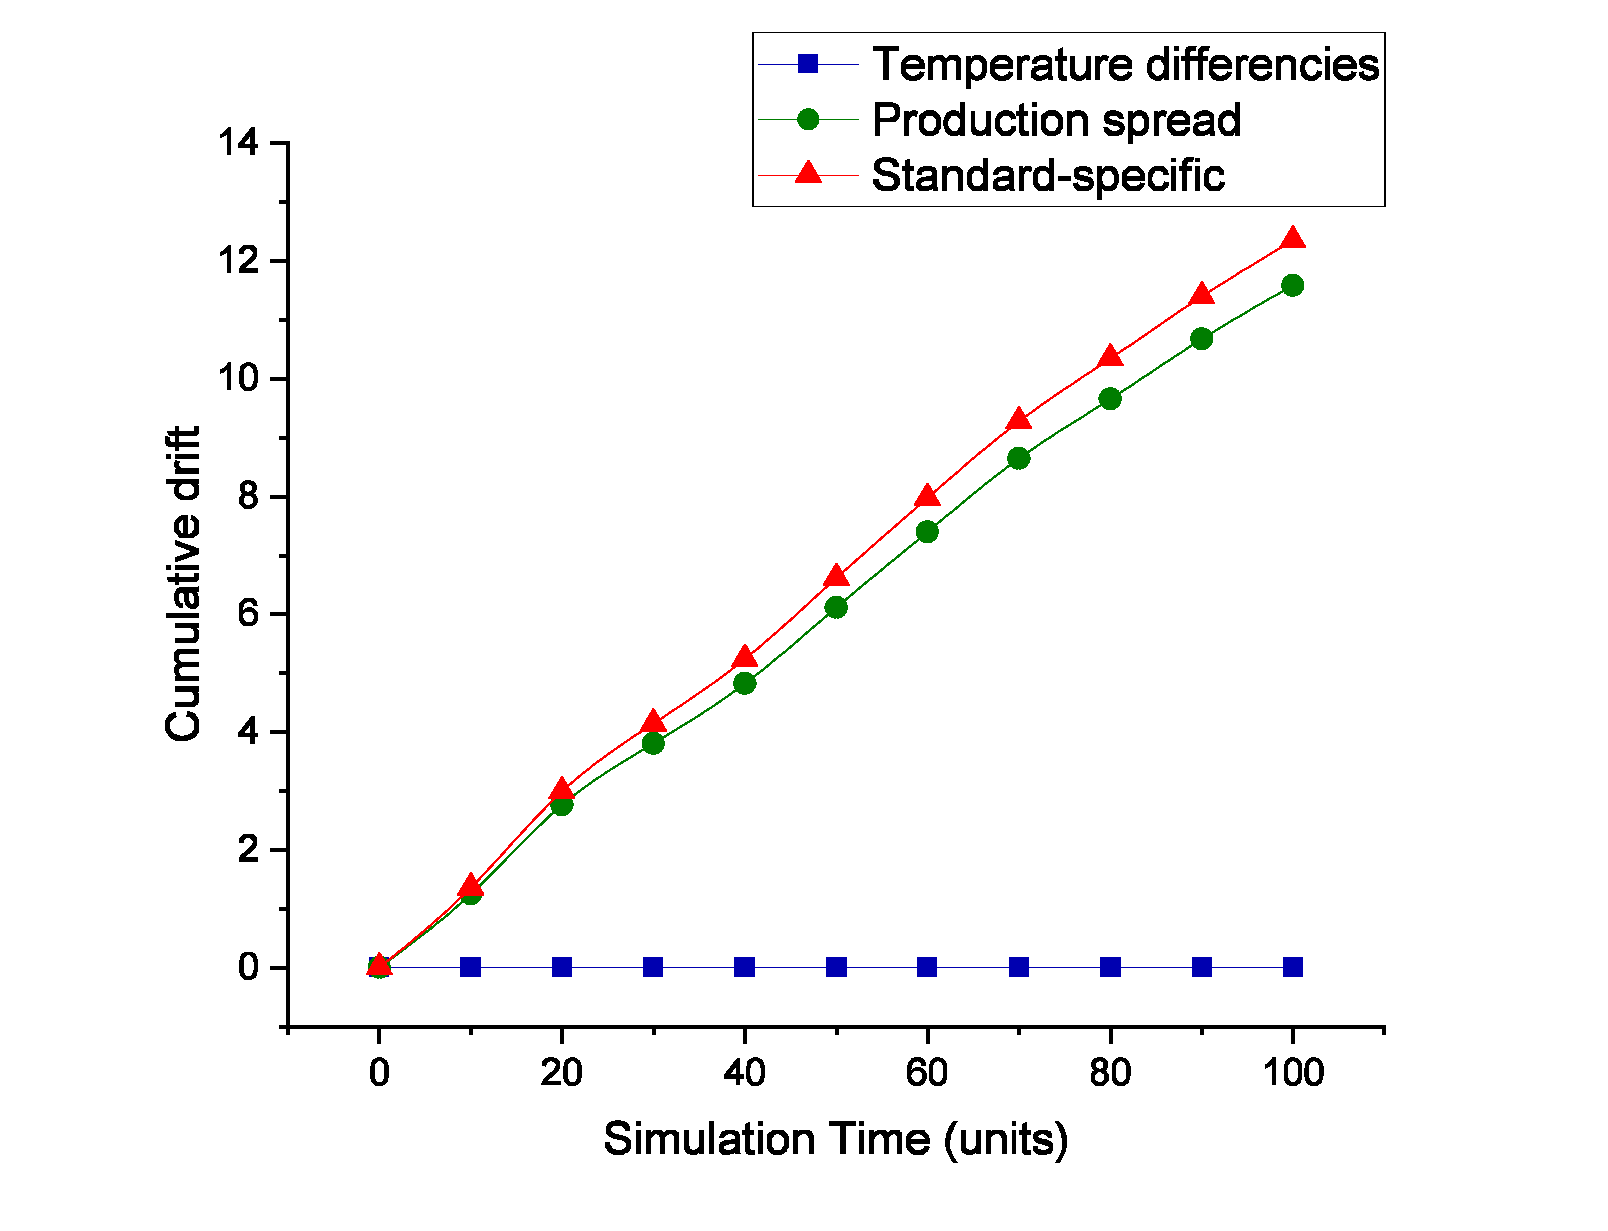
\includegraphics[width=340pt, height =220pt]{driftclock.pdf}
    \caption{Cummulative Effects od desynchronization.}
    \label{fig:usecase:cranes:graphic:plot:desynch}
\end{figure} 




Considering the updated model \quot{\eclipse{M3}} incorporating drifting monitoring  through probabilistic commands and gateway synchronization, we will verify property \ref{eq1} while varying \texttt{d1proba} and \texttt{d2proba} within the range \texttt{[0,1]} with increments of \texttt{0.1}. The resulting model checking results are portrayed in \fig{fig:01} and \fig{fig:02} during variation of the probabilistic variable \texttt{d1proba} and probabilistic variable \texttt{d2proba}, respectively. 

\noindent
    \begin{figure}[!htb]
    \centering
       \begin{tabularx}{\linewidth}{ m{8cm}   m{8cm}  }
           
\noindent
 \begin{minipage}[t]{8cm}
     \centering

    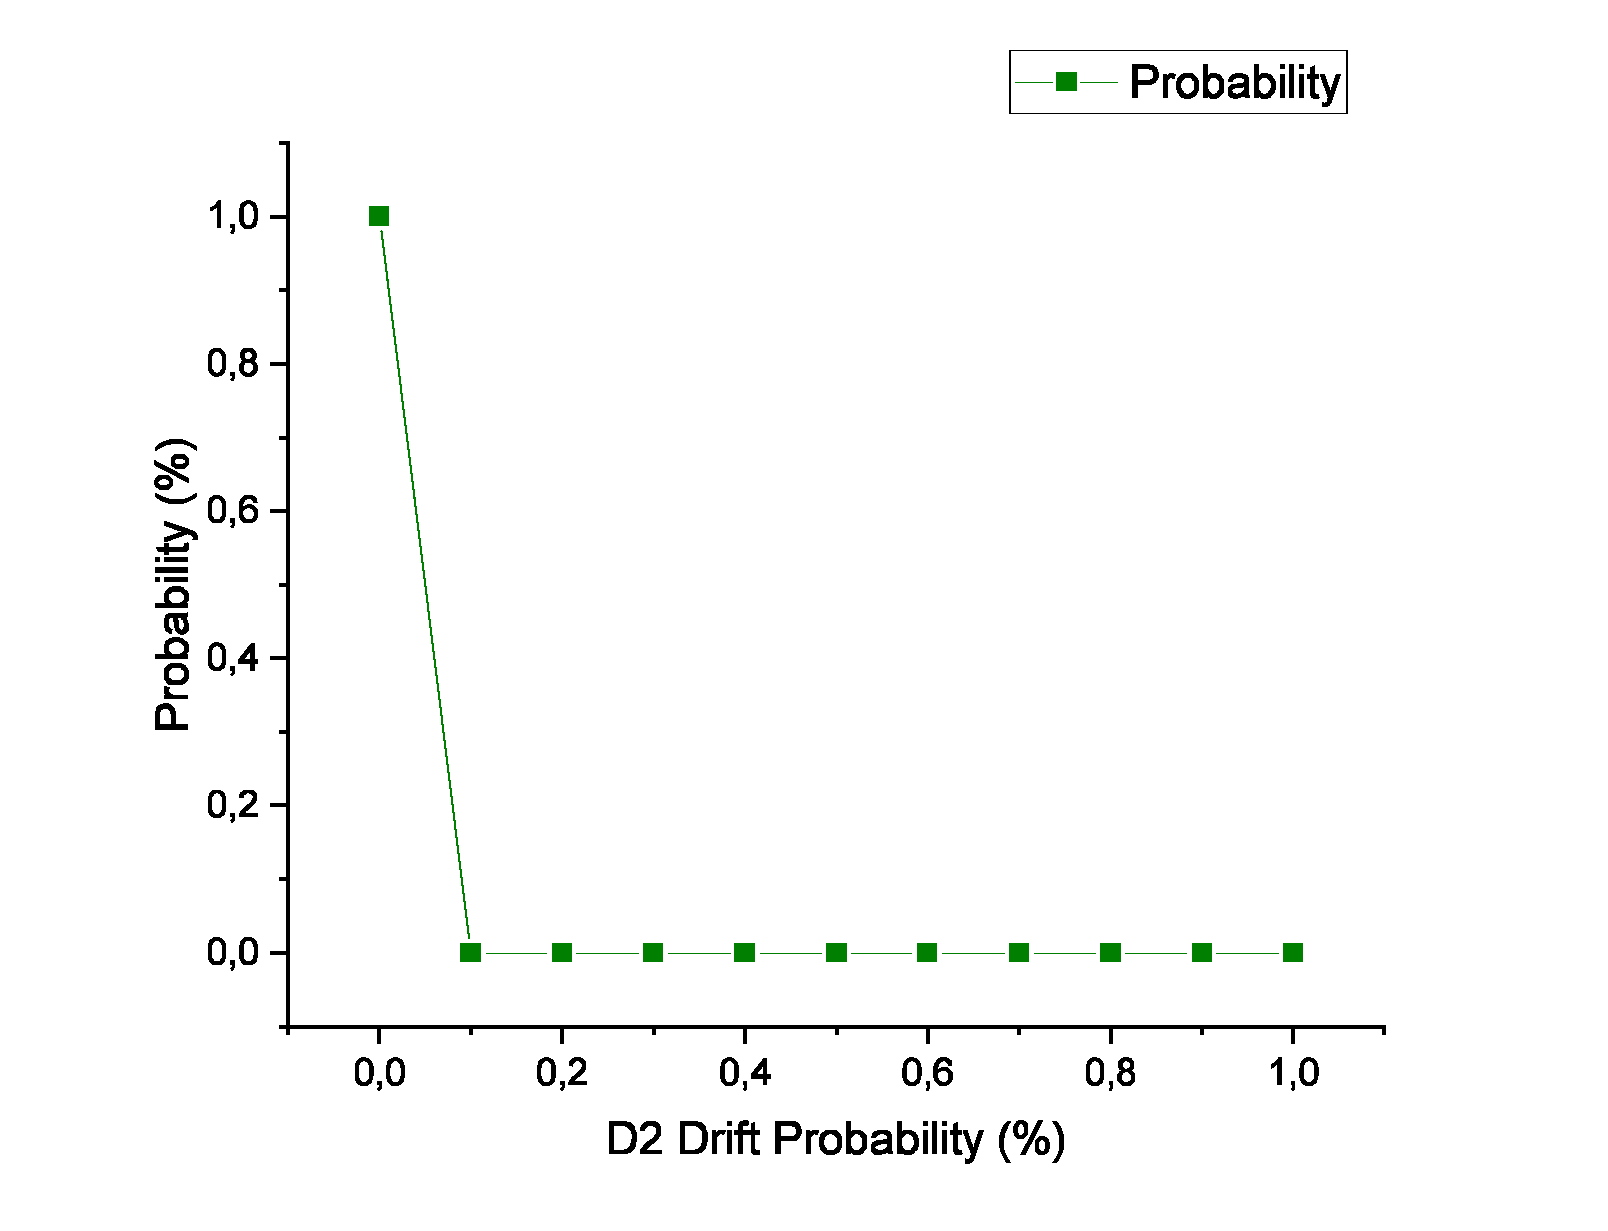
\includegraphics[width=180pt, height =140pt]{Graph1.pdf}
    \caption{Verification of Property \ref{eq1} with Drift variation on D2.}
    \label{fig:01}
   \end{minipage}
    
           &
\noindent
   \begin{minipage}[t]{8cm}
     \centering
   		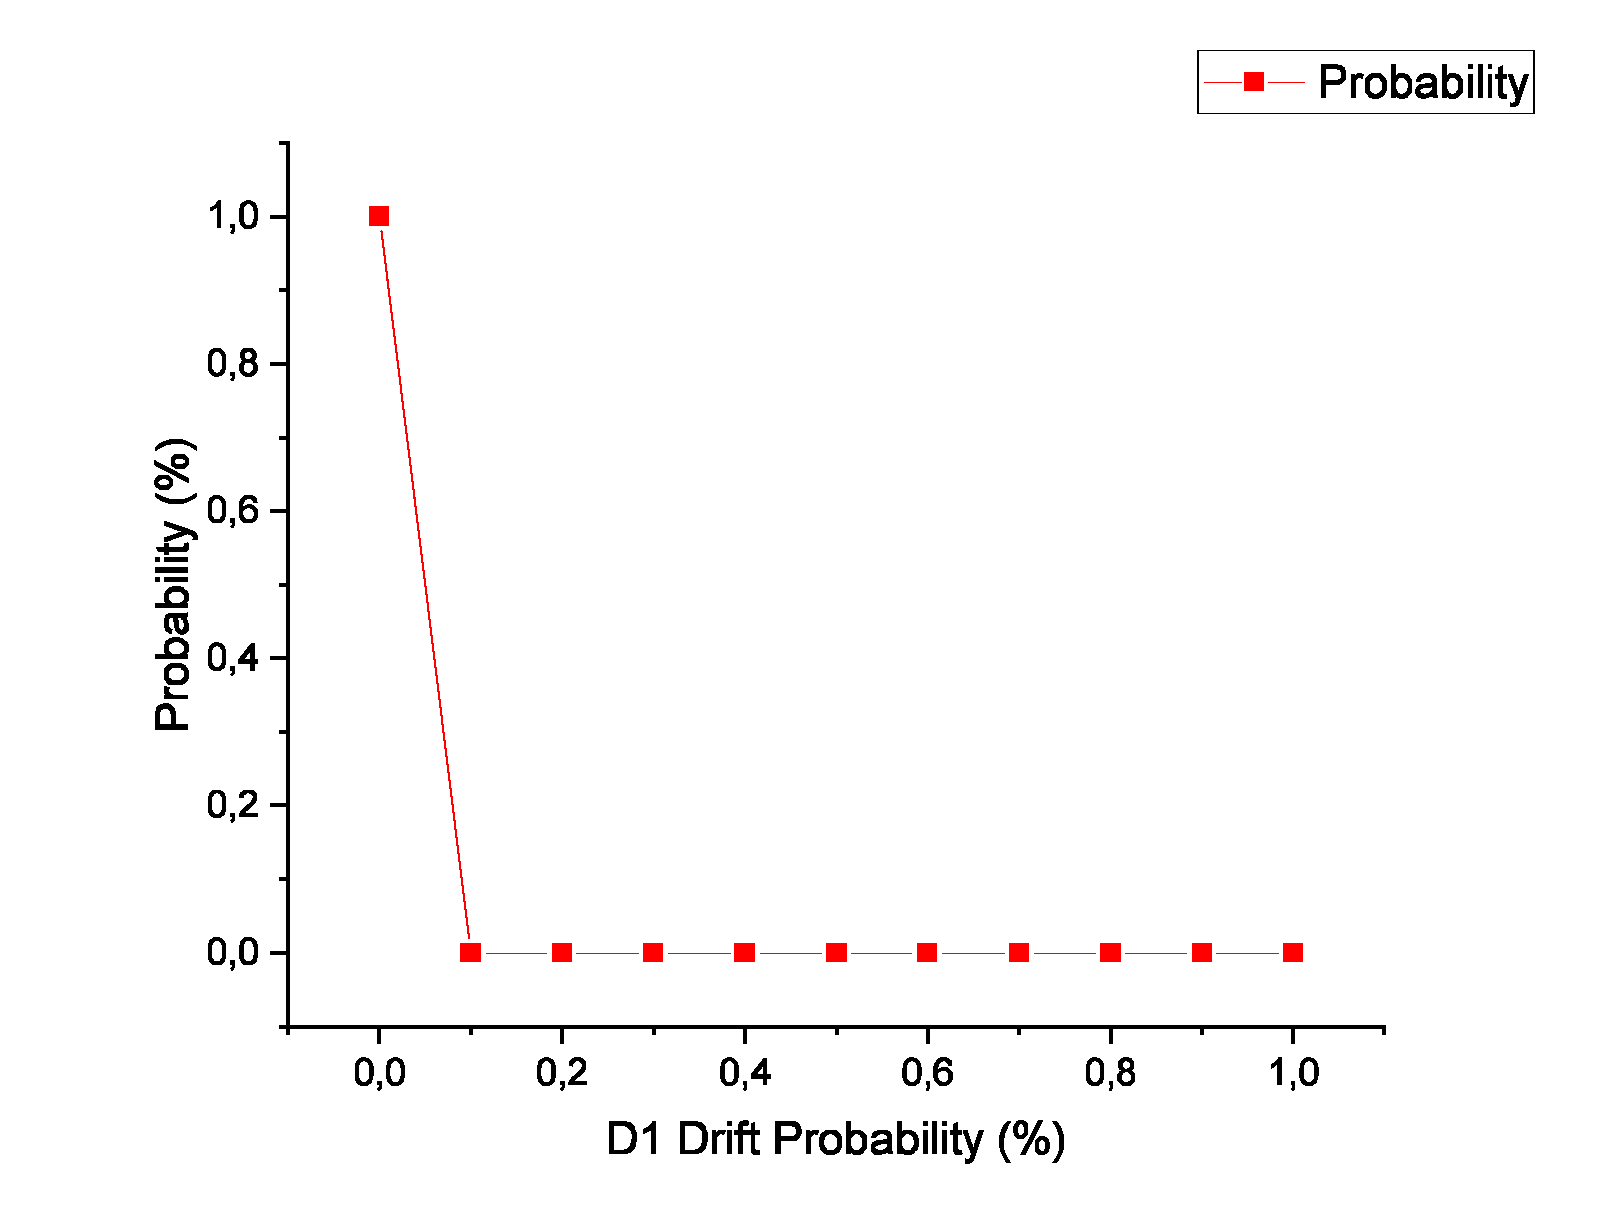
\includegraphics[width=200pt, height =140pt]{Graph2.pdf}
    \caption{Verification of Property \ref{eq1} with Drift variation on D1.}
    \label{fig:02}
   \end{minipage}

       \\ 
    
           \end{tabularx}
\end{figure}

The graphs in \fig{fig:01} and \fig{fig:02} demonstrate that if the drones' local clocks drift with different values, the property is not satisfied with a probability greater than \texttt{0\%}. This implies that the property cannot be guaranteed using the global operator alone. To ensure synchronization through the gateway, we define the following property:

\begin{framed}
\emph{\bfseries{Property3}}: The system eventually reaches a state where both drones (D1 and D2) are synchronized after desynchronization.
\end{framed}



	    \begin{resp}{\textbf{\textit{Property3}}}
        \begin{equation}
        \label{eq2}
         \mathtt{ P=? [ \  \ !(\textcolor{red}{D1H}==\textcolor{red}{D2H}) \implies \ F \ (\textcolor{red}{D1H}==\textcolor{red}{D2H}) \  ]} 
        \end{equation}
        \end{resp}
        \normalsize






Checking the property \ref{eq2} while varying \texttt{d1proba} and \texttt{d2proba} within the range \texttt{[0,1]} with increments of \texttt{0.1} under synchronization. The resulting model checking results are portrayed in \fig{fig:03} and \fig{fig:04} during variation of the probabilistic variable \texttt{d1proba} and probabilistic variable \texttt{d2proba}, respectively. The results show that during system execution, in spite, of the local clock time drifts,  the gateway performs resynchronization with a probability of \texttt{100\%}. 

        \noindent
    \begin{figure}[!htb]
    \centering
       \begin{tabularx}{\linewidth}{ m{8cm}   m{8cm}  }
           
\noindent
 \begin{minipage}[t]{8cm}
     \centering

    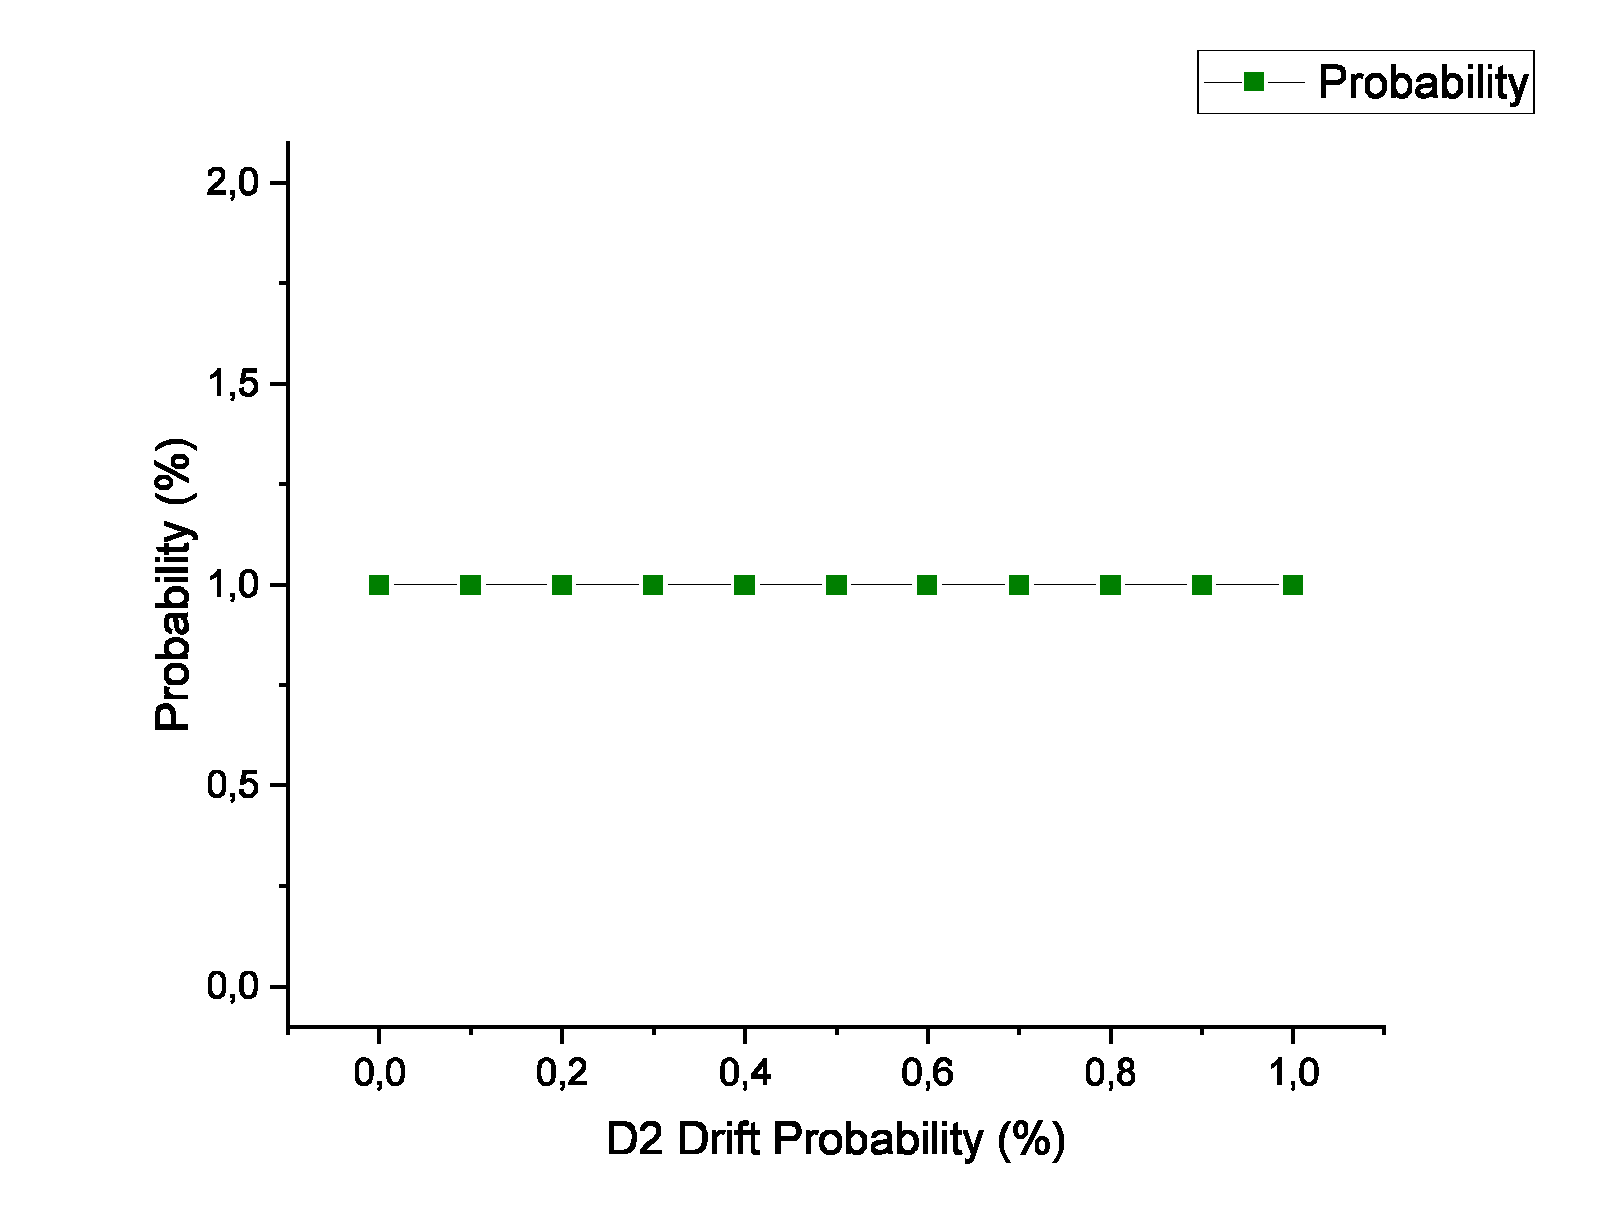
\includegraphics[width=180pt, height =140pt]{Graph4.pdf}
    \caption{Verification of Property \ref{eq2} with Drift variation on D2.}
    \label{fig:04}
   \end{minipage}
    
           &
\noindent
   \begin{minipage}[t]{8cm}
     \centering
   		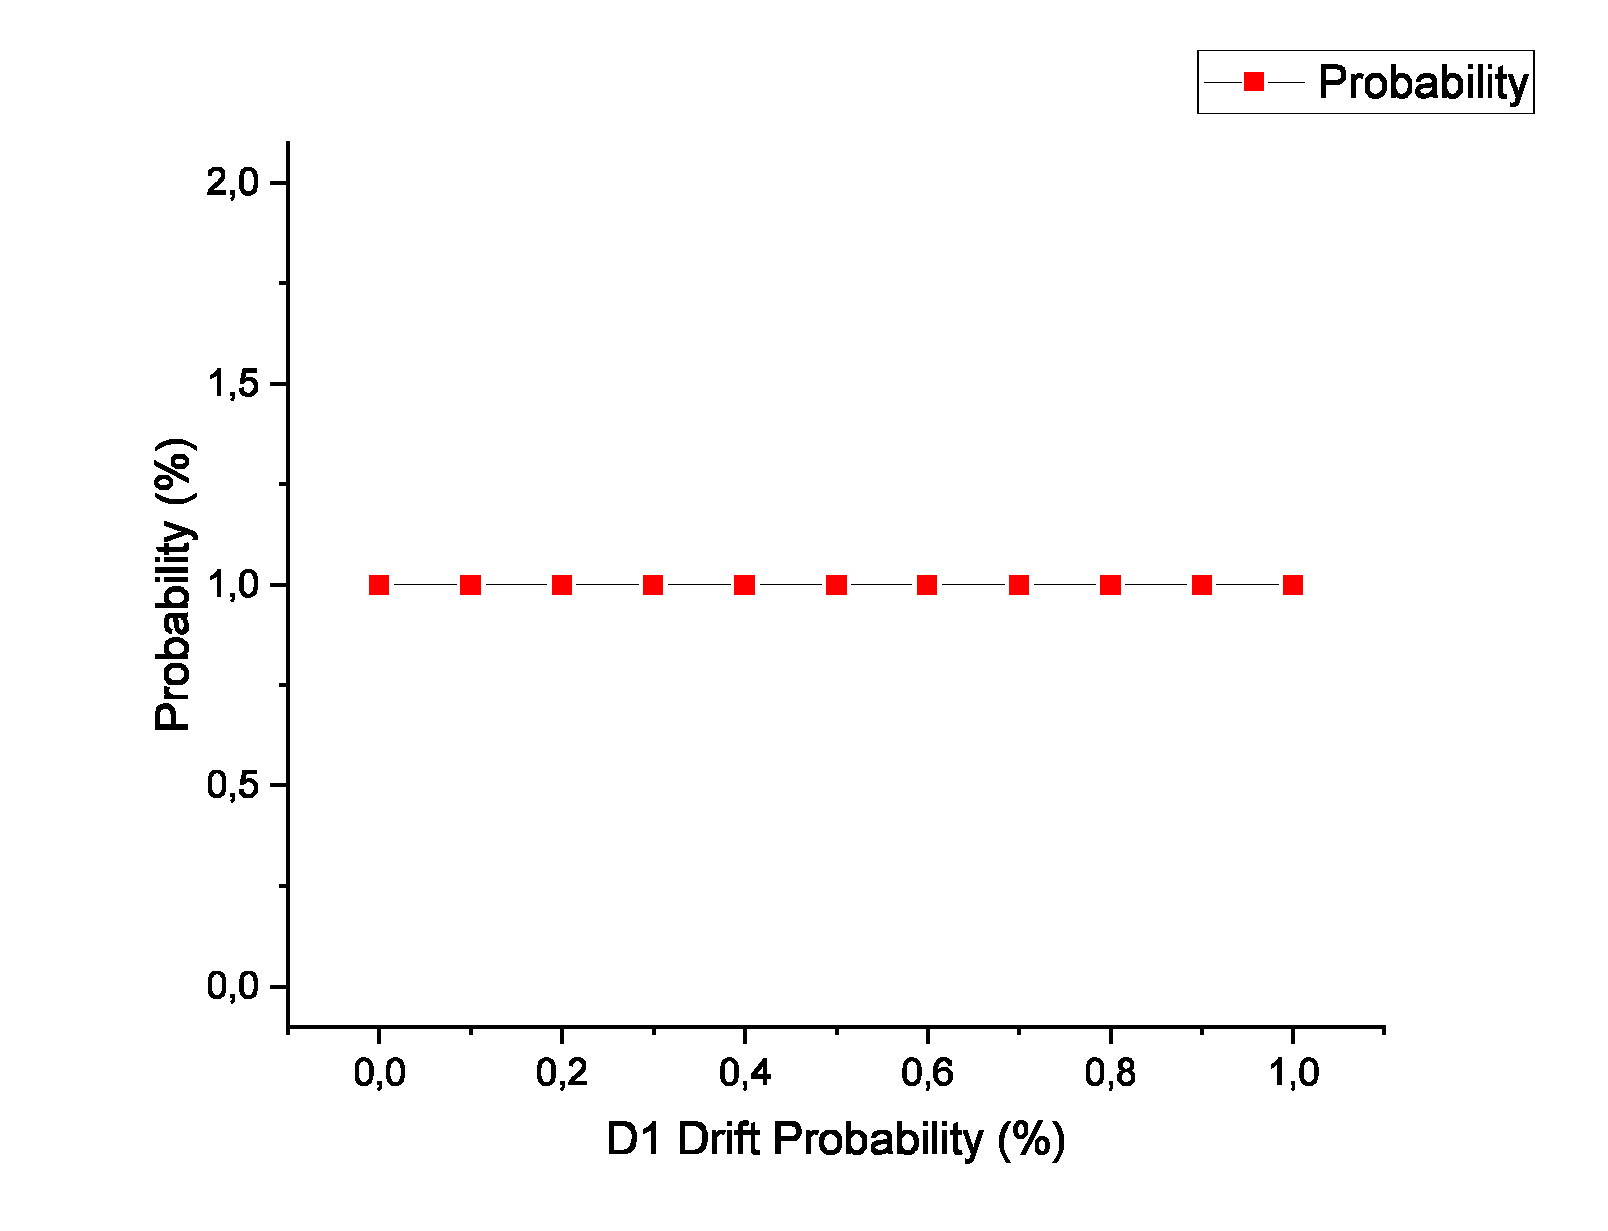
\includegraphics[width=200pt, height =140pt]{Graph03.pdf}
    \caption{Verification of Property \ref{eq2} with Drift variation on D1.}
    \label{fig:03}
   \end{minipage}

       \\ 
    
           \end{tabularx}
\end{figure}

\lstset{
    breaklines=true,
    style=framed,
    escapeinside={<@}{@>},
    morekeywords={void, int, public, private, class, protected, submodules, network, connections, const, init, int, bool, double, module, rewards, endrewards, endmodule},
    basicstyle=\ttfamily,
    keywordstyle=\bfseries\color{blue},
        morecomment=[f][\color{green!30!black}][0]{/*},
    morecomment=[l][\color{green!30!black}]{//},
    label=queueemodel
}



\begin{figure}[!htb]            
\begin{minipage}{16.5cm}
\begin{lstlisting}[style=framed,%customc,
	caption=PRISM Code for Clock Drift Observation,
 	label=modelparameters]	
...
module D1
...
D1cycleLength : [0..MAXH] init 13;

D1refractoryPeriod : [0..MAXH] init 6;

D1nextBroadcast : [0..MAXH] init NEXT_BROADCAST;
...
endmodule
\end{lstlisting}
 \end{minipage}  
\end{figure}

\paragraph{Limitations} While the modeled system using PRISM can handle up to \emath{10^{9}} states, this capacity is still a limitation. Despite setting boundaries on model variables, such as those defined in the first drone module (lines 4-8 of the code snippet \lst{modelparameters}), the model encounters state space explosion. For example, the variable \texttt{D1cycleLength} is restricted by the global variable \texttt{MAXH}, which is set to 15 units. This approach effectively reduces the state space compared to an open-boundary model, which would exacerbate the challenge faced by many model checkers. Another challenge arises not from model construction but from the property being verified. This property is based on liveness, as defined by \citeauthor{alur2015} \cite{alur2015}. This is a common experience in model checking, where a specific (and potentially complex) algorithm is required to verify the model against the property. One of the solutions that is provided in this paper falls in the scope of model checking by validation.









\subsection{Design and validation through simulation using OMNeT++}
To address the problems encountered in the previous section, designers can model systems using OMNeT++, which leverages C/C++ but requires knowledge of component-based programming. Algorithms~\ref{algo:model:algo:figo} and~\ref{algo:model:algo:inbox} are implemented in C/C++ code. However, the model architecture components denoted as \emath{\mathcal{ND}} (See section \ref{omnet} ), are constructed using OMNeT++ language constructs. The code snippet in \lst{omnetusecase} portrays the architecture of the use case. The model without and with synchronization using inbox gateway is available on \cite{csi2023} referenced as \quot{\eclipse{C1}} and \quot{\eclipse{C2}}, respectively.

\lstset{
    breaklines=true,
    style=framed,
    escapeinside={<@}{@>},
    morekeywords={void, int, public, input, output,private, class, protected, submodules, network, parameters, gates, simple, connections, const, init, int, bool, double, module, rewards, endrewards, endmodule},
    basicstyle=\ttfamily,
    keywordstyle=\bfseries\color{blue},
        morecomment=[f][\color{green!30!black}][0]{/*},
    morecomment=[l][\color{green!30!black}]{//},
    label=queueemodel
}


\begin{figure}[!htb]            
\begin{minipage}{16.5cm}
\begin{lstlisting}[style=framed,%customc,
	caption=Architecture of Cranes Lifting Orchestration via Drones,
 	label=omnetusecase]	
simple Drone //Drone component 
{
    parameters:
        double driftRate;
    gates:
        input DRONE_LISTEN;
        output DRONE_TRANSMIT;
        output CRANE_LIFT;
}

simple InBox // gateway component
{ 
    gates:
        input DRONE0_TRANSMIT;
        input DRONE1_TRANSMIT;
        output DRONE0_LISTEN;
        output DRONE1_LISTEN;
}

simple Crane //crane component
{
    gates:
        input CRANE_LIFT;
}

network CranesOrchestration //architecture composition
{
  submodules:
      Drone0: Drone { }
      Drone1: Drone { }
      Gateway: InBox {  }
      Crane0: Crane { }
      Crane1: Crane { }
 connections:
  Drone0.DRONE_TRANSMIT --> {  delay = 100ms; } --> Gateway.DRONE0_TRANSMIT;
  Drone1.DRONE_TRANSMIT --> {  delay = 100ms; } --> Gateway.DRONE1_TRANSMIT;

  Gateway.DRONE0_LISTEN --> {  delay = 100ms; } --> Drone0.DRONE_LISTEN;
  Gateway.DRONE1_LISTEN --> {  delay = 100ms; } --> Drone1.DRONE_LISTEN;

  Drone0.CRANE_LIFT --> {  delay = 100ms;} --> Crane0.CRANE_LIFT;
  Drone1.CRANE_LIFT --> {  delay = 100ms; } --> Crane1.CRANE_LIFT;
}
\end{lstlisting}
 \end{minipage}  
\end{figure}

The OMNeT++ architecture is characterized by three simple modules (i.e. \emath{\mathcal{ND}}components) (other complex components can be deployed depending on the complex architecture). The modules are characterized by parameters and gates. Parameters are initial variables defined by the OMNeT++ user. In our case \texttt{driftRate} refers to the drifting value collected from the hardware and environmental characteristic (see Section \ref{drifting}) to make our model flexible and parametrizable. Gates using the keyword \texttt{gates} refers to the \emath{\mathcal{ND}} component port.  Data can be exchanged by broadcasting (using \texttt{output} port) or receiving through this port (using \texttt{input} port) on lines 6-8, lines 14-17, and line 23.



The OMNeT++ system composition is defined by the network configuration in lines 26-43. The \emath{\mathcal{ND}} components are instantiated as submodules (using the keyword submodules) in lines 29-33. During this instantiation, additional configuration parameters like icons can be specified.

Communication between components is established through connections configured using the keyword \texttt{connections}. For example, the \texttt{DRONE\_TRANSMIT} output gate of the Drone module is connected to the \texttt{DRONE0_TRANSMIT} input gate of the \texttt{InBox} module. Lines 35-42 define other connections between component gates. Communication can be delayed by specifying a value for the delay parameter. For instance, a 100-millisecond delay can be set for connections.

\noindent
\begin{figure}[!htbp]
    \centering
    		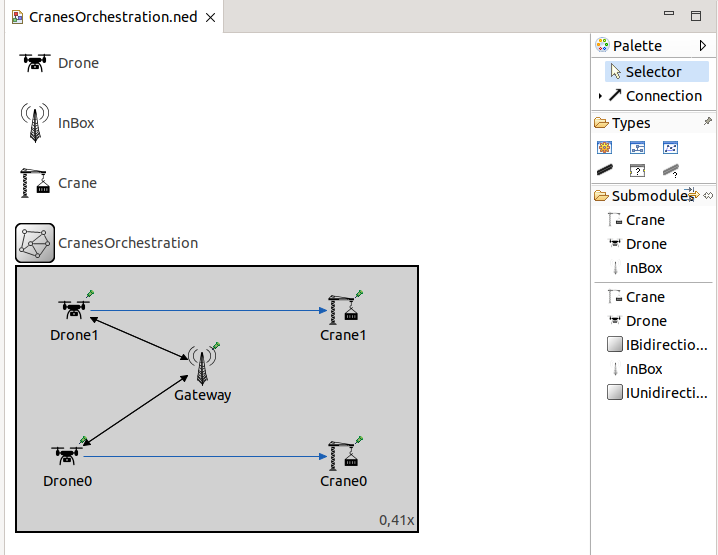
\includegraphics[width=350pt, height =250pt]{graphic.png}
    \caption{Cranes Lifting Orchestration via a Drone using OMNeT++ Graphical Tool. }
    \label{fig:usecase:cranes:graphic}
\end{figure} 


The graphical representation of the network architecture is shown in \fig{fig:usecase:cranes:graphic}. On the right side, you'll find various modules available for instantiating additional \emath{\mathcal{ND}}components. This tool promotes reusability by allowing the definition of reusable modules, providing a flexible configuration option common in most simulation tools. Additionally, designers can enhance the architecture's clarity for non-expert designers by adding icons to different components.



\lstset{
    breaklines=true,
    style=framed,
    escapeinside={<@}{@>},
    morekeywords={void, int, public, if, else, virtual, input, output,private, class, protected, submodules, network, parameters, gates, simple, connections, const, init, int, bool, double, module, rewards, endrewards, endmodule},
    basicstyle=\ttfamily,
    keywordstyle=\bfseries\color{blue},
        morecomment=[f][\color{green!30!black}][0]{/*},
    morecomment=[l][\color{green!30!black}]{//},
    label=queueemodel
}


\begin{figure}[!htb]            
\begin{minipage}{16.5cm}
\begin{lstlisting}[style=framed,%customc,
	caption=Drone Component Functions,
 	label=omnetusecasedrone]	
    class Drone : public cSimpleModule
    {
    public:
        Drone();
    private:
        cMessage*  TRANSMIT;
        double driftRate; // drift rate in seconds
        int H;
        int PLD;
        int nextBroadcast;
        int cycleLenght;
        int refractoryPeriod;
        int sameCount;
        const int  sameThreshold=2;
        std::exponential_distribution<double> distribution;
        void transmit(int H, int pld);
   protected:
        // The following redefined virtual function holds the algorithm.
        virtual void initialize() override;
        virtual void handleMessage(cMessage *msg) override;
    };
\end{lstlisting}
 \end{minipage}  
\end{figure}

\begin{figure}[!htb]            
\begin{minipage}{16.5cm}
\begin{lstlisting}[style=framed,%customc,
	caption=C/C++ Code Internal Component Structure,
 	label=omnetusecasedronefunction]	
void Drone::initialize()
{
    driftRate = par("driftRate");
}
void Drone::handleMessage(cMessage *msg)
{
...
    if(H==cycleLenght){
        H=0;
        sameCount=0;
    }else{
        double interval = distribution(generator,std::exponential_distribution<double>::param_type(driftRate));
        if (interval <= driftRate) {
            H=H+2;
        } else {
            H=H+1;
        }
    }
}
void Drone::transmit(int H, int pld)
{
    ...
    TRANSMIT = new cMessage(result.c_str());
    send(TRANSMIT, "DRONE_TRANSMIT"); // send out the message
  }
\end{lstlisting}
 \end{minipage}  
\end{figure}

The internal structure of the drone component is defined using a class in C/C++. This class encapsulates the drone's behavior through a set of attributes (data) and functions (methods). An example code snippet for the drone component is provided in the \lst{omnetusecasedrone}. The parameters referring to the drift \texttt{driftRate} are defined as a double value. The \texttt{driftRate} is assigned its initial value during simulation setup using the par function within the \texttt{initialize} function (lines 1-4) of the \lst{omnetusecasedronefunction}.

The \texttt{handleMessage} function (lines 5-19) in \lst{omnetusecasedronefunction} is responsible for processing incoming messages. For example, it can collect complex messages for internal computations based on previously defined algorithms. However, drift is handled differently in our implementation (line 12). We use the \texttt{distribution} function to calculate an interval at which the simulation generates a drift value based on the \texttt{driftRate}  parameter. If the interval is greater than the \texttt{driftRate}, the local clock is incremented by 2 units. Otherwise, it is incremented by 1 unit. It is important to note that OMNeT++ offers specific libraries for managing drift. However, these libraries might limit designer control over the implementation.

The \texttt{transmit} function handles the transmission of messages in \texttt{string} format, adhering to the OMNeT++ message structure declared on line 6 of \lst{omnetusecasedrone}. It achieves this by invoking a predefined function, \texttt{send}, which is responsible for communicating the message through the designated port, \texttt{DRONE\_TRANSMIT}. The designers have to configure the structure of the string message with the relevant data during the processing.


Validation is achieved through simulation within the OMNeT++ environment. The simulator depicts packets originating from drones and their transmission to the gateway clock synchronization. Finally, the system instructs cranes to initiate lifting operations. The source code is publicly available, enabling academic and industry readers to download and interact with the simulator. Users can manipulate the animation speed by accelerating or decelerating it for a customized experience. However, this paper focused on collecting specific values from the gateway, including the input drone clock values and the generated clock values used for synchronization. \cmt{Communication lag is a critical factor in synchronization, the clock H and payload Pld messages are sent first to the gateway before to the drones. In our current work, estimating the non-exploitable time during model checking is performed within the simulation scenario. This estimation focuses on the number of messages sent by drones and collected by the gateway. Using the simulator, we assess how synchronization impacts communication delays, resulting in a delay range of [0.3; 21.3] seconds. The developed OMNeT++ code incorporates the computation of communication lag.}


The generated CSV file containing a collection of monitored drones' internal clocks is available online (see \cite{csi2023}). Users can access and consult this data for further analysis. The file is produced by custom C/C++ code that appends data entries to the CSV file. Each entry follows a specific header structure, including simulation time, the first drone's clock value, the second drone's clock value, and the synchronized value. \fig{fig:usecase:cranes:graphic:plot:synch} depicts a snapshot of the different internal clock values (lines blue and green). By analyzing this figure, we can observe that the synchronization process (red line) occurs periodically, coinciding with each captured instance of desynchronization. This validation proves the accuracy of the algorithm in running synchronization.

\noindent
\begin{figure}[!htbp]
    \centering
    		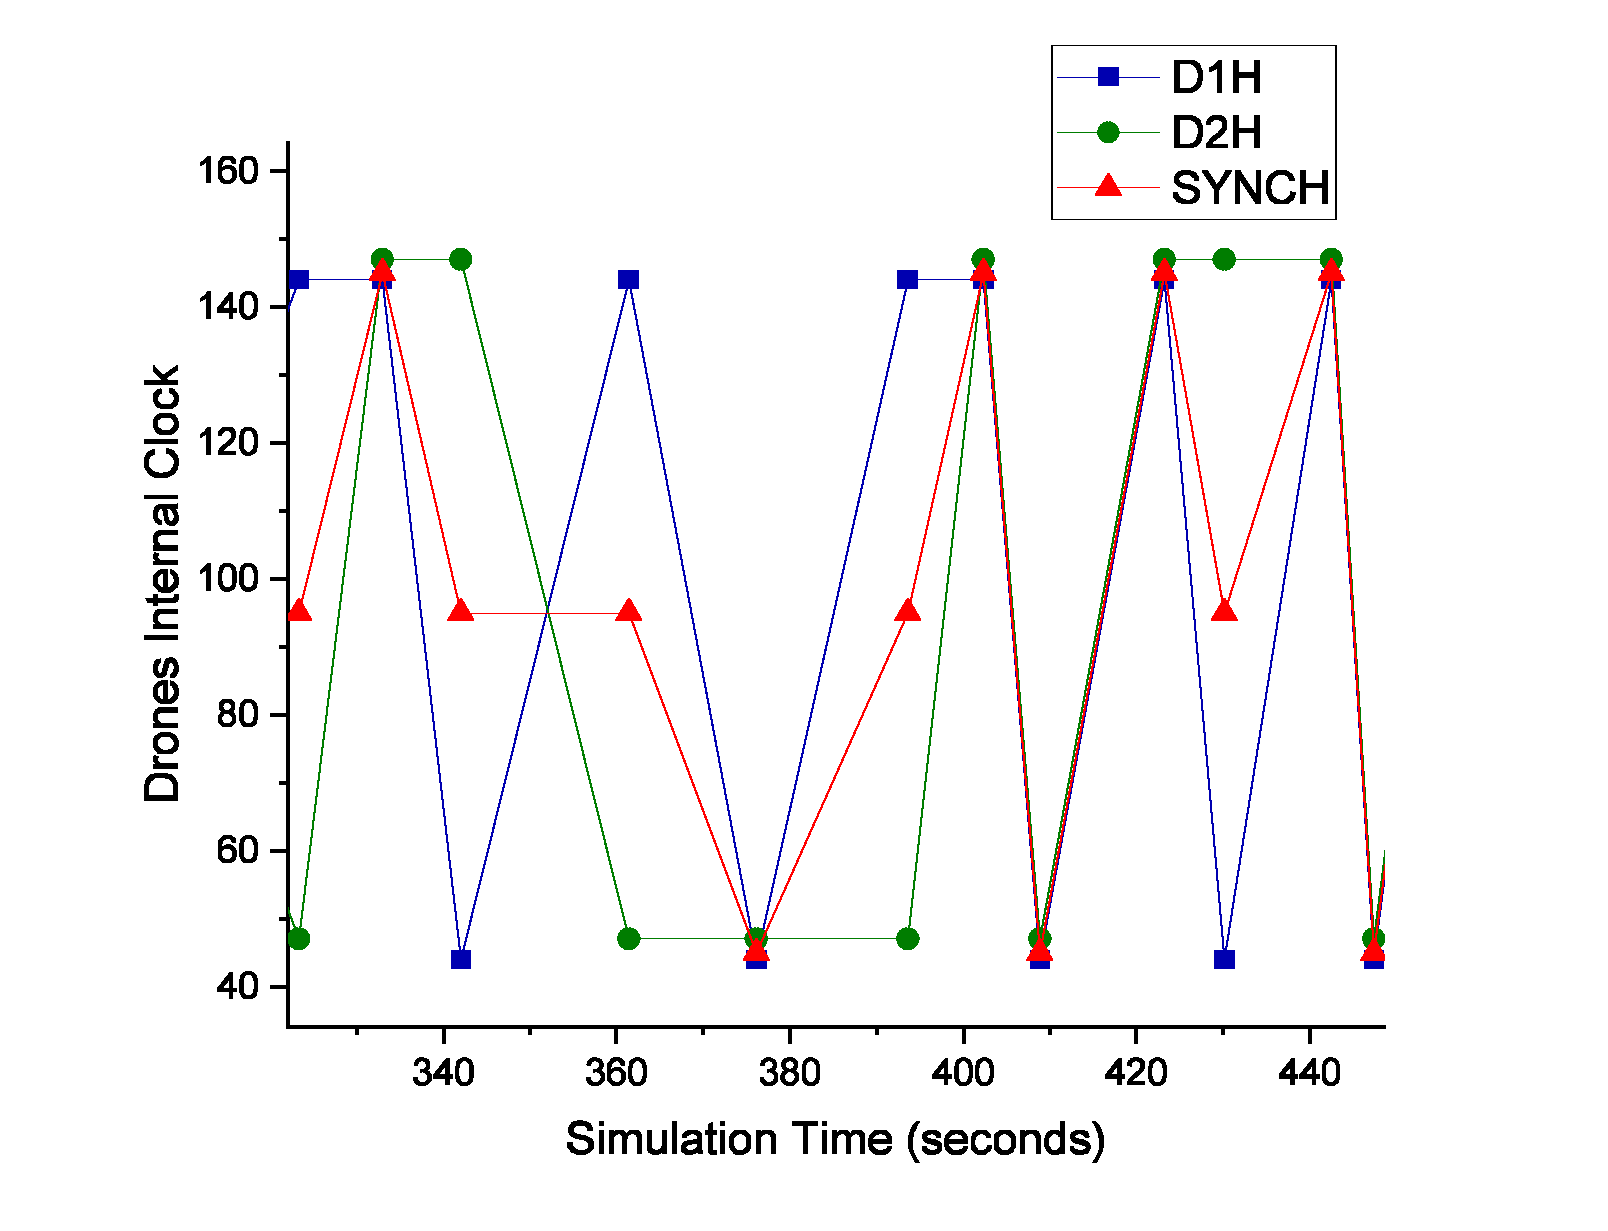
\includegraphics[width=340pt, height =220pt]{GraphDrones.pdf}
    \caption{Plotting Internal Clock Synchronization for Model under Temperature Variations.}
    \label{fig:usecase:cranes:graphic:plot:synch}
\end{figure} 



To assess the validation accuracy, we employed a PDT. First, we trained the decision tree on the previously generated CSV file. This tree learns relationships between features (e.g., D1H and D2H) and synchronized drone clock constraint outcomes in the form of classes. For example, when considering the clock drift caused by temperature variations as discussed in \cite{WEBSTER2020101183} (see \fig{fig::synch:pdt} for the decision tree visualization), the tree would classify data points based on clocks values and predict the corresponding synchronized outcome. The decision tree has three synchronization classes, labeled from 0 to 2. The root node splits data based on a constraint on the feature \texttt{D2H}. The second-level nodes further refine the classification using constraints on \texttt{D1H} values. Finally, the leaf nodes assign data points to the corresponding synchronization classes. The relevant Python code can be found in \cite{csi2023} under the model reference \eclipse{P2}. 

\noindent
\begin{figure}[!htbp]
    \centering
    		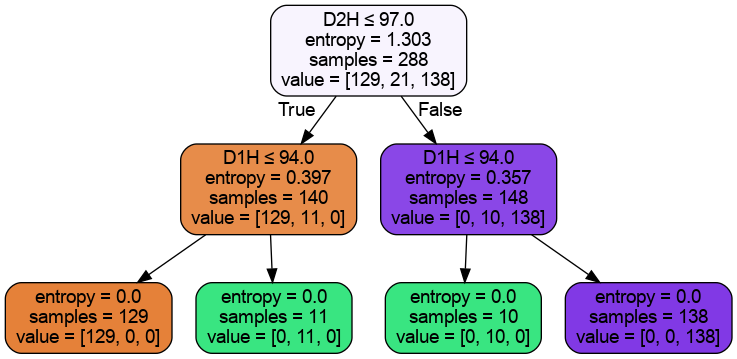
\includegraphics[width=360pt, height =190pt]{decisiontree.png}
    \caption{Generated Decision Tree from CSV File .}
    \label{fig::synch:pdt}
\end{figure} 


\subsection{From decision trees to probabilistic commands}

\lstset{
    breaklines=true,
    style=framed,
    escapeinside={<@}{@>},
    morekeywords={void, int, public, private, class, protected, submodules, network, connections, const, init, int, bool, double, module, rewards, endrewards, endmodule},
    basicstyle=\ttfamily,
    keywordstyle=\bfseries\color{blue},
        morecomment=[f][\color{green!30!black}][0]{/*},
    morecomment=[l][\color{green!30!black}]{//},
    label=queueemodel
}



\begin{figure}[!htb]            
\begin{minipage}{16.5cm}
\begin{lstlisting}[style=framed,%customc,
	caption=Mapping to Probabilistic Commands for Model under Temperature Variations,
 	label=learnedprismmodel]	
dtmc  // This line declares the model as a Markov Decision Process (MDP)

// Constant definitions
const int NOTDEFINED = -1; // Defines a constant value for "not defined"
const double D1H;       // Declares a constant double variable named D1H
const double D2H;       // Declares a constant double variable named D2H

// Module definition
module GeneratedDecisiontree  // Defines a module named GeneratedDecisiontree

  // State variable
  CL : [NOTDEFINED..3] init NOTDEFINED;  // Declares a state variable named C with a range of [NOTDEFINED, 3] and initial value 0 to identify a set of classes

  // PRISM rules
  [rule1] D2H <= 97.0 & D1H <= 94.0 ->  (0.007751937984496124) : (CL' = 0) + (0.9922480620155039) : (CL' = NOTDEFINED);  // Probability (0.9922...) for setting C' to NOTDEFINED

  [rule2] D2H <= 97.0 & D1H > 94.0 ->  
    (0.09090909090909091) : (CL' = 1) +  
    (0.9090909090909091) : (CL' = NOTDEFINED);

  [rule3] D2H > 97.0 & D1H <= 94.0 ->  
    (0.1) : (CL' = 1) +  
    (0.9) : (CL' = NOTDEFINED);

  [rule4] D2H > 97.0 & D1H > 94.0 ->  
    (0.007246376811594203) : (CL' = 2) +  
    (0.9927536231884058) : (CL' = NOTDEFINED);

endmodule  // End of module definition

\end{lstlisting}
 \end{minipage}  
\end{figure}

The decision tree generated in \fig{fig::synch:pdt} is translated into a set of PRISM commands shown in \lst{learnedprismmodel}. The PRISM model uses three constant global variables: \texttt{NOTDEFINED}, \texttt{D1H}, and \texttt{D2H}. The first variable, initialized to -1 in line 4, represents an undefined class state. The other variables (D1H and D2H), defined in lines 5-6, are initialized by the user during model checking. The generated classes are identified by the state variable C (line 12). This variable can take values from -1 to 3. Since the decision tree generates three classes, class 0 corresponds to a value of 0, and class 2 corresponds to a value of 2. By default, the variable is initialized to NOTDEFINED (-1).

The first rule (line 15) defines a constraint on \texttt{D1H} and \texttt{D2H}. If \texttt{D2H} is less than 97 time units and \texttt{D1H} is less than 94 time units, then the state variable CL is assigned class 0 with a probability of 0.007. Otherwise, CL is assigned the \texttt{NOTDEFINED} class with a probability of \texttt{0.99}. This constraint pattern is repeated in subsequent commands (lines 17-25).

Now consider the definition of the stochastic model generated by mapping the decision trees to PRISM commands. The properties expressed here will differ from those previously discussed. The following property is expressed in natural language as:


\begin{framed}
\emph{\bfseries{Property4}}: After the drones transmit their clock ticks to the gateway, the generated synchronization class is expected to fall within the interval [0, 2].
\end{framed}



	    \begin{resp}{\textbf{\textit{Property4}}}
        \begin{equation}
        \label{eq3}
         \mathtt{ P=? [ \ G( \ !(\textcolor{red}{D1H}==\textcolor{red}{D2H}) \implies \ F \ (\textcolor{red}{CL}\geq 0 \& \textcolor{red}{CL}\leq 2) \ ) ]} 
        \end{equation}
        \end{resp}
        \normalsize

Verifying Property~\ref{eq3} shows a \texttt{100\%} probability that the synchronization will be achieved based on drifting categories in section \ref{drifting}: Temperature Variations, Standard-Specific Drift, and Production Spread, starting from an initial state with unsynchronized internal clocks. Such a result confirms the efficiency of the algorithm regarding the different parameter variations.

\subsection{Computational aspects of models scalability}
The PRISM models referenced as \quot{\eclipse{M1}} to \quot{\eclipse{M6}} in \cite{csi2023} suffer from the problem of state space explosion, as discussed previously in the context of model checking limitations. This issue stems from the liveness properties and the way they are verified by the supported engines. Our solution is to model the system in OMNeT++ as \quot{\eclipse{C2}} in \cite{csi2023}. We then generate the corresponding dataset to train decision tree rules, which are then used to build a more tractable model. In this context, we present a model architecture that scales from two drones to six drones. We then compare the time it takes to construct and verify these models regarding property \ref{eq3}. This comparative analysis will provide insights into the limitations of model checking for validation, particularly regarding scalability.


We constructed a model based on the decision trees generated from the data. This model was then replicated for three clusters. Each cluster represents the structure of two drones and three cranes. We verified the model against Property \ref{eq3}. Finally, we measured the time to construct the model and the time to perform verification, considering both the computed states and transitions. In Table \ref{tableTime} we portray the evaluation of the developed model \quot{\eclipse{M6}} and the scaled models \quot{\eclipse{M7}}, \quot{\eclipse{M8}}, and \quot{\eclipse{M9}} in \cite{csi2023}. These models exhibit different characteristics regarding the number of states, transitions, model construction time, and model verification time. The reference model, for example, exhibits a high number of states and transitions. This captures the complexity of the algorithms' structure and the use of variable numbers. However, models \quot{\eclipse{M7}}, \quot{\eclipse{M8}}, and \quot{\eclipse{M9}} demonstrate fewer states and transitions, making them more suitable for timely verification. Verifying the reference model on two clusters took a very long time without producing any results, despite the computational power of the execution machine.






\begin{table}[h!]
\centering

\begin{tabular}{|c c c c c c |} 
\hline 
Model ID & NB Cluster & States & Transitions & Model Construction & Model Checking\\
\hline
\eclipse{M3} & Reference Model & 149533 & 387244 & 2.245 seconds & 1.643 seconds\\
\eclipse{M7}& 1 & 2 & 4 & 0.001 seconds  & 0.003 seconds\\
\eclipse{M8}& 2 & 4& 12 & 0.004 seconds  & 0.039 seconds\\
\eclipse{M9}& 3 & 8 & 32 & 0.031 seconds & 0.002 seconds \\
\hline 
\end{tabular}
\caption{Computational Aspects of Models Scalability.}
\label{tableTime}
\end{table}


According to the reference paper~\cite{Wang2006}, the verification cost is defined as 1 - (\emath{\frac{Tv(\mathcal{P}_{2})}{Tv(\mathcal{P}_{1})}}) and abstraction efficiency is defined as 1 - (\emath{\frac{Tc(\mathcal{P}_{2})}{Tc(\mathcal{P}_{1})}}). We refer by \emath{\mathcal{P}_{1})} to the reference model (\quot{\eclipse{M3}}) while we refer by \emath{\mathcal{P}_{2})} to models in  \quot{\eclipse{M7}}, \quot{\eclipse{M8}}, and \quot{\eclipse{M9}}. The function \emath{Tv} computes the model verification time and the function \emath{Tc} computes the model construction time. Computation times are collected from the PRISM model checker verification engine.


In this case, the model construction efficiency is very high at \texttt{0.999}. This indicates that constructing the abstract model takes significantly less time compared to the reference model. Similarly, the verification cost of \texttt{0.998} suggests that verifying the abstract model is also faster. However, the reference model with multiple clusters cannot be verified and doesn't provide any results. To address this limitation, we introduce the concept of a limit function. This concept allows the verification and construction times to approach 1, indicating very efficient processing in model construction and verification.


\subsection{Threats to validity}
In the following section, we identify and highlight the potential threats associated with our experimentation that may arise during the infrastructure deployment. 

Since the dataset was generated by an OMNeT++ simulator rather than a real-world infrastructure, the collection process might not fully capture parameters relevant to physical deployment. This raises the possibility of outliers and potentially meaningless data, requiring careful handling during analysis.

The dataset was collected from the OMNeT++ gateway component, where we specifically captured data at that level. Consequently, experiments with similar models that include gateways are likely. However, the chosen component for data collection might limit the experiment's monitoring to gateways and not other network components.